\section{Supplementary Appendix}

\subsection{Influencer Recruitment}
\label{app:inf_recruit}

\begin{table}[ht]
\centering 
\caption{Distribution of social media influencers according to recruitment strategy \label{tab:reports_tab}}
\begin{tabular}{llcccc}\\
  \toprule
  \multicolumn{2}{c}{ } & \multicolumn{4}{c}{Recruitment Criteria} \\
\cmidrule(l{3pt}r{3pt}){3-6} 
 Phase & Country & Both & Only Popularity & Only News Sharing  & Twitter Ads  \\
\midrule
Pilot & Kenya & 20 & 0 & 0 & 0 \\ 
& South Africa & 20 & 0 & 0 & 0 \\ 
&&&&&\\ 
First Batch & Kenya & 47 & 11 & 18  & 0\\ 
& South Africa & 14 & 34 & 28 & 0 \\ 
&&&&&\\
Second Batch & Kenya & 3 & 2 & 4 & 49\\ 
& South Africa & 3 & 21  & 12  & 16\\ 
\midrule
Mean [Followers] &  & 31,497.551 & 14,607.706 & 2,873.952 & 10,985.446 \\ 
Std. Dev. [Followers] &  & 55,361.358 & 18,352.048 & 695.712 & 30,804.893 \\ 
  \bottomrule \multicolumn{6}{l} {\parbox[t]{16cm}{ \scriptsize{\textit{Notes:} This table presents the distribution of social media influencers at each phase and country separating by recruitment criteria. Column 1 and 2 refers to the phases of the intervention and country of origin of the influencers. Column 3-7 present the number of influencers obtained by each inclusion criteria. Column 3 shows influencers that complied with both the popularity and high-quality news sharing criteria, meaning those influencers that shared at least one high-quality news or fact check and with more than 4,490 followers in Kenya and more than 3,265 followers in South Africa. Column 4 shows all influencers with more than the average number of followers in each country but that did not share any news or fact checks. Column 5 shows all influencers that shared at least one news or fact check and had more than 2,000 followers but less than the average number of followers in each country. Column 5 shows all influencers recruited through Twitter Ads.}}}
\end{tabular}
\end{table}



%%%%%%%%%%%%%%%%%%%%%%%%%%%%%% ML Models

\newpage 

\subsection{Inferring the Verifiability of Twitter and Facebook Posts Using BERT}
\label{ver_bert}

To construct a training data set, we identified and scraped the viral posts in English from three African countries: Nigeria, Kenya and South Africa, and sent them to Africa Check. Africa Check fact-checkers labeled 1,000 of these viral posts as \textit{Not Verifiable}, \textit{Verifiable}, and \textit{Somewhat Verifiable}. The initial distribution of these labels was as follows. Out of the thousand posts, 477 (47.7\%) were labeled as not verifiable, 158 (15.8\%) as somewhat verifiable, and 365 (36.5\%) as verifiable. To augment this data set and have a more balanced data set in terms of verifiability, we incorporated 121 verified Twitter posts and 96 Facebook posts fact-checked by Africa Check and thus inherently verifiable. The final distribution of labeled posts is portrayed in Table~\ref{tab:ver1}. \\

\begin{table}[ht]
\centering
\caption{Distribution of 1,217 labeled posts:3 labels \label{tab:ver1}}
\begin{tabular}{lccc}\\
  \hline
Type & Label & Number & Percent  \\ 
  \hline
\textit{Not Verifiable} & 1 & 477 & 0.39  \\ 
\textit{Somewhat Verifiable} & 2 & 158 & 0.13  \\ 
\textit{Verifiable} & 3 & 582 & 0.48  \\ 
   \hline
\end{tabular}
\end{table}

To develop an algorithm capable of accurately and automatically predicting the verifiability of the multitude of posts we handled daily, we tried on leveraging cutting-edge NLP models of the time (which likely still are). In our specific scenario, we opted for BERT, a deep learning model built on the robust Transformers architecture. Having been trained on millions of data points this model had already learnt the inner structure of the English language and its features can be used to train a standard classifier. Following the relevant literature at the moment, we chose the same optimization and loss functions. For the optimization function we used AdamW, since the results are generally better than every other optimization algorithm, have faster computation time, and require fewer parameters for tuning (\cite{Kingma-2017}, \cite{Ruder-2016}). For Binary Classification problems, we use the Binary Cross-Entropy as a loss function, which is the go-to loss function for these types of problems, since the cross-entropy error function is often used for classification problems when outputs are interpreted as probabilities of membership in an indicated class (\cite{Reed}; \cite{Goodfellow-et-al-2016}). \\

After training the first few models and failing to obtain one that could distinguish between the \textit{verifiable} and \textit{somewhat verifiable} classes, we decided to pool them together into one single class and train a binary classifier instead. The resulting distribution of labeled posts is portrayed in Table~\ref{tab:dist2}. Finally, upon trying several hyper-parameters we decided on the model which had validation (out of sample) accuracy of 85$\%$ and cross-validation accuracy of 84$\%$. This model included a DropOut regularizer and a linear activation function, we also decided to leave the stop-words since BERT could utilize them to understand context better. The confusion matrix in Figure~\ref{fig:ver2} shows this more clearly.

\begin{table}[ht]
\centering
\caption{Distribution of 1,217 labeled posts: 2 labels \label{tab:dist2}}
\begin{tabular}{lccc}\\
  \hline
Type & Label & Number &  Percent \\ 
  \hline
\textit{Not Verifiable} & 0 & 477 & 0.44  \\ 
\textit{Verifiable} & 1 & 600 & 0.56 \\ 
   \hline
\end{tabular}
\end{table}

\begin{figure}[h]
    \centering
    \caption{Verifiability Model: Confusion matrix \label{fig:ver2}}
    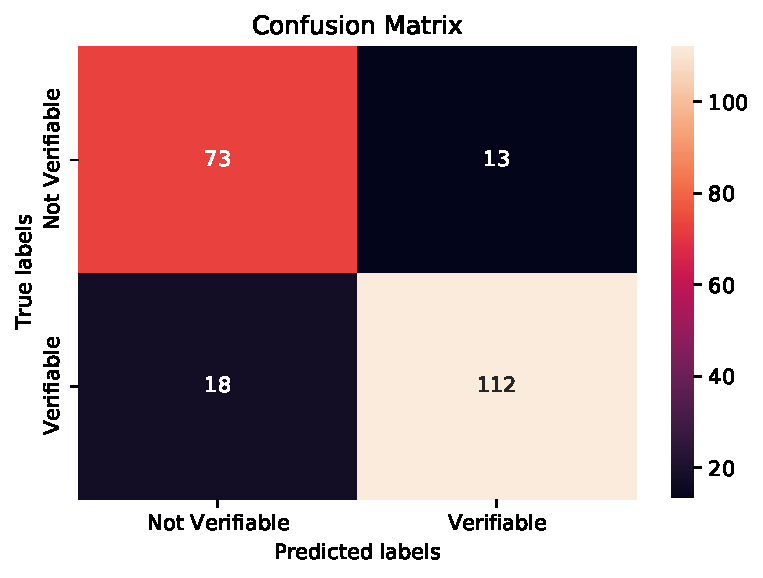
\includegraphics[width=10cm, height=9cm]{../results/desc_stats/cm_bert_2class_linear_drop3.pdf}
\end{figure}

\newpage

\subsection{Fake News Detection of Twitter and Facebook Posts Using BERT}
\label{fake_bert}

Over the years, Africa Check has manually verified thousands of posts deemed fake news and stored some of them alongside the prediction made. Out of these posts, we could recover the text from 456, which were all (except for two) classified as fake news. To add true posts and gain balance between fake and true posts, we built a data set containing around 100 thousand newspaper Tweets from the three most reliable sources in Nigeria (Mobile Punch), Kenya (Standard Kenya), and South Africa (Daily Maverick)\footnote{As recommended by the Chief Editors at AfricaCheck.}. From this 100 thousand Tweets, filtered out non-relevant Tweets related with opinions, sponsored content and business reviews and randomly sampled 30 thousand Tweets from each newspaper.\\

We further matched 456 of them to the fake ones using matching and natural language processing techniques that allowed us to identify which true post was closest to a fake one in terms of the topics they covered (identified in an automated way) and common words used in each topic.  This balanced data set, not only label-wise but also topic-wise, reduces the association between fake news and certain topics, which is usually time-dependent and affects fake news labeling outside the period of the data set. To do this we employed a LDA Topic Model\footnote{A better description of the model and the results can be found in Appendix \ref{lda_fake}}, with 5 Topics, which was fitted into the fake training data provided by Africa Check and used to predict and match on the newspaper data.

We augmented this data set with 600 political posts scraped from the FakeNet DataSet, which is a data set of US news Tweets labeled as true or fake. The label distribution of the training is in Table~\ref{tab:fake1}.

\begin{table}[ht]
\centering
\caption{Distribution of 1,518 labeled posts \label{tab:fake1}} 
\begin{tabular}{lccc}\\
  \hline
Type & Label & Number & Percent \\ 
  \hline 
\textit{Fake} & 0 & 692 & 0.456  \\ 
\textit{True} & 1 & 826 & 0.544  \\ 
   \hline
\end{tabular}
\end{table}

As with the verifiability model, after training several models using BERT, we decided on the one model which had the highest test (out of sample) accuracy, as reflected in the following confusion matrix in Figure~\ref{fig:fake2}.\\

\begin{figure}[!htpb]
    \centering
    \caption{Fake model: Confusion matrix \label{fig:fake2}}
    \label{fig:fig2}
    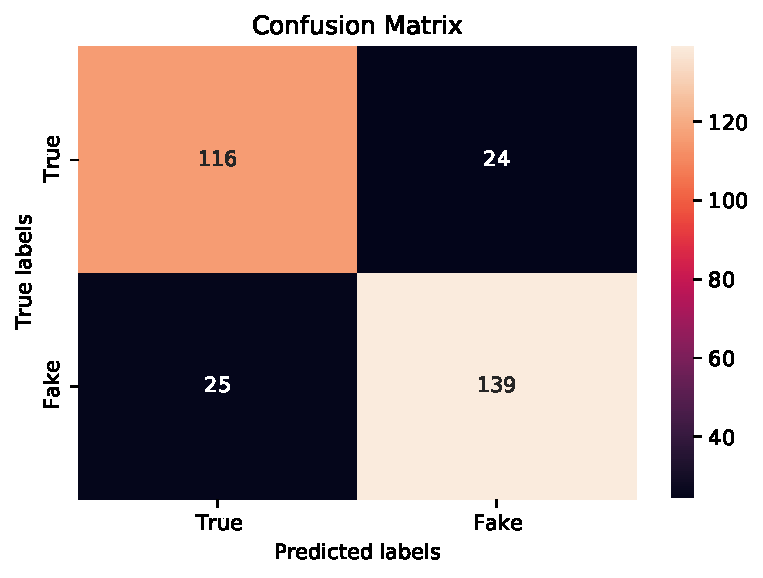
\includegraphics[width=10cm, height=8cm]{../results/desc_stats/fake_bert_linear_drop.pdf}
\end{figure}

For both models we checked the cross-validation accuracy to discard that our results were influenced by the size of our training data set and/or the sampling to split training and validation. For both cases we obtained validation accuracies close to 85$\%$, which ruled out any concern about the validity of the results.\\


\subsection{Topic modeling}

\subsubsection{LDA model: fake dataset}
\label{lda_fake}

Latent Dirichlet Allocation (LDA) is a probabilistic generative model widely employed in the field of natural language processing for topic modeling. LDA posits that documents are generated from a distribution over latent topics, with each topic characterized by a distribution of words. The model's generative process entails the assignment of topics to words in documents, guided by prior distributions \cite{Blei-LDA}\footnote{Given the timing of the deployment of the experiment, compared to when we analyzed the results of it, a few other models came into seen, like BERTopic.}. 

In our experiment, we utilized the Latent Dirichlet Allocation (LDA) model to analyze the topics present in our fake dataset. We then applied this model to predict the topics in a large collection of authentic posts gathered from reputable newspapers across Africa. After making these predictions, we compared the topic distributions of each post using a method called cosine similarity. By doing so, we were able to find the most similar authentic post for each fake post based on their topic distributions. This approach allowed us to pair each fake post with a genuine counterpart that closely matched in terms of the topics discussed.\\

We started looking at some objective measures of good fit, such as the Coherence and the Perplexity. Coherence measures the semantic similarity between high-frequency words within a topic. It helps assess how interpretable and meaningful the topics are. It is calculated by considering pairs of words that frequently co-occur within documents. A higher coherence score indicates that the words in a topic tend to be more closely related in meaning. Therefore, a good coherence score suggests that the model has successfully identified coherent topics that capture distinct themes present in the corpus \cite{CohMeasure}. On the other hand, the perplexity score measures how well the model predicts the observed documents in the dataset. A lower perplexity score indicates better predictive performance.\\

The evaluation of LDA models based solely on coherence and perplexity scores may not provide a complete understanding of which model is a better fit. As seen in Table \ref{tab:coherence}, although the scores across both dimensions are relatively similar, the model with 9 topics exhibits superior performance. However, upon closer examination of each model's relevant words, we observed that the model with 5 topics produced the most human-interpretable results. It became apparent that in models with a relatively high number of topics, there was a tendency for repeated keywords across multiple topics, indicating that the value of 'k' (the number of topics) might be too large. Furthermore, with an increase in the number of topics, their interpretability diminishes, making it more challenging to discern meaningful distinctions between them.\\

\begin{table}[H]
\caption{Topic Coherence and Perplexity across Different Models}
\centering
\label{tab:coherence}
\begin{tabular}{|c|c|c|}
\hline
Topics & Perplexity & Coherence\\
\hline
4 & -8.463 & 0.414\\
5 & -8.558 & 0.420\\
6 & -8.673 & 0.430\\
7 & -8.765 & 0.430\\
8 & -8.775 & 0.440\\
9 & -8.799 & 0.440\\
\hline
\end{tabular}
\end{table}

Given these, we decided to stick to the 5 Topic Model, since it yielded the most humanly interpretable topics. These topics, as we can see in Figure \ref{fig:LDAmodel}, are related with Economic conditions in Africa (Topic 1), Political context (Topic 2), health misinformation related with traditional medicine (Topic 3) and health misinformation related with modern medicine (Topic 5).

\begin{figure}[htbp]
    \centering
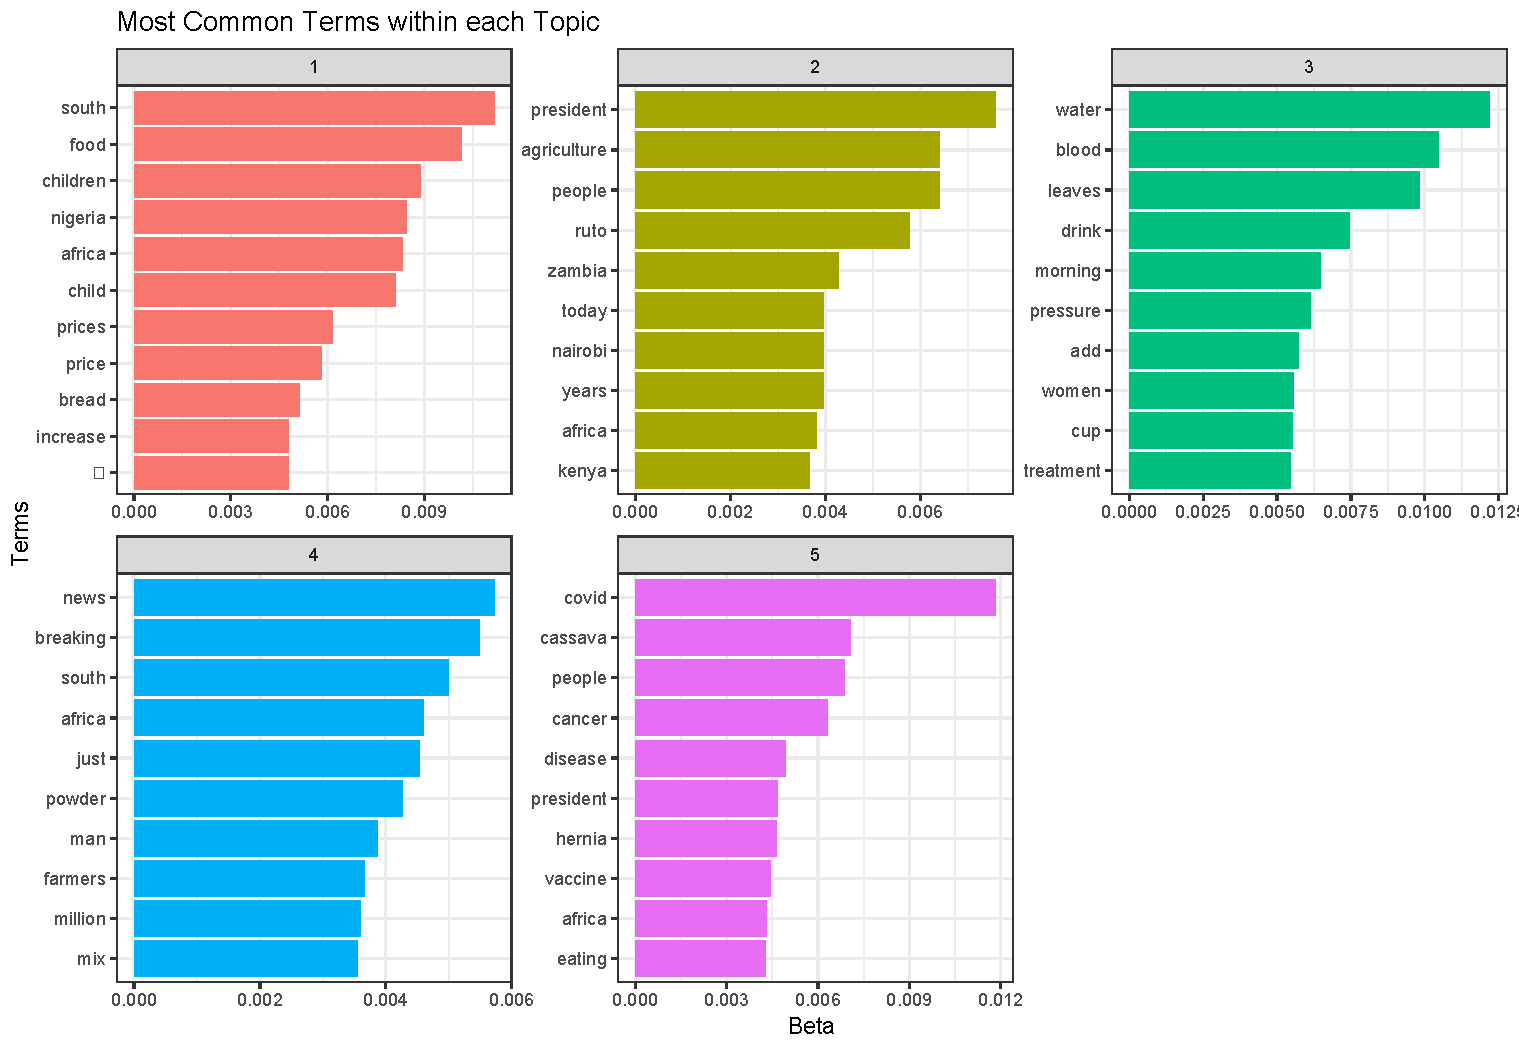
\includegraphics[width=0.98\textwidth]{../results/desc_stats/5Topics.pdf} 
        \caption{LDA Model 5 Topic Word Scores} 
    \label{fig:LDAmodel}
\end{figure}

\newpage

\subsection{COVID sentiment analysis}
\label{app:covid_bert}
Given that the information influencers posted to their followers was heavily related to COVID-19 and vaccination campaigns, an interesting outcome we analyzed was the change in sentiment towards these topics. Due to the large number of Tweets to be analyzed, we decided to use machine learning algorithms to automate the sentiment prediction of the Tweets.

We obtained a training data set from \href{https://www.kaggle.com/datasets/datatattle/covid-19-nlp-text-classification}{Kaggle}. This dataset is human-labeled and contains Tweets from all of 2020 regarding COVID-19. It has 5 labels: Extremely Positive, Positive, Neutral, Negative and Extremely Negative. For practical reasons we pooled together these 5 labels into three, Positive, Neutral and Negative. The data set is divided in training (41,157 observations) and test (3,798). Given the number of training points we have, we decided to fully balance the data set. So for our model with 3 classes we have 18,046 observations for each one of them.

For our main analysis\footnote{We also use VADER for robustness of results.}, we used a BERT (Bidirectional Encoder Representations from Transformers) model, specifically we fine-tuned the \href{https://huggingface.co/bert-base-uncased}{bert-base-uncased} and added and train a classifier layer on top of the BERT architecture. This BERT model is significantly bigger than the Small BERT (over 108 million parameters). After 5 training epochs we obtained the following metrics.

We obtained 92\% of validation accuracy and a test accuracy of 89\%, calculated by the F-Score metric. Moreover, we see no major bias in any of the classes from the confusion matrix in Figure \ref{fig:conf_BERT_base}, meaning that the model does not confuse any of the classes of has issues predicting on a particular one. Also, by looking at the learning curve in Figure \ref{fig:lc_BERT_base} we see no concern regarding over-fitting and under-fitting, which we solved through several iterations and trying different set of regularizers and even the Small BERT.

\begin{figure}[H]
    \centering
    \caption{Learning Curve: BERT Base}
    \label{fig:lc_BERT_base}
    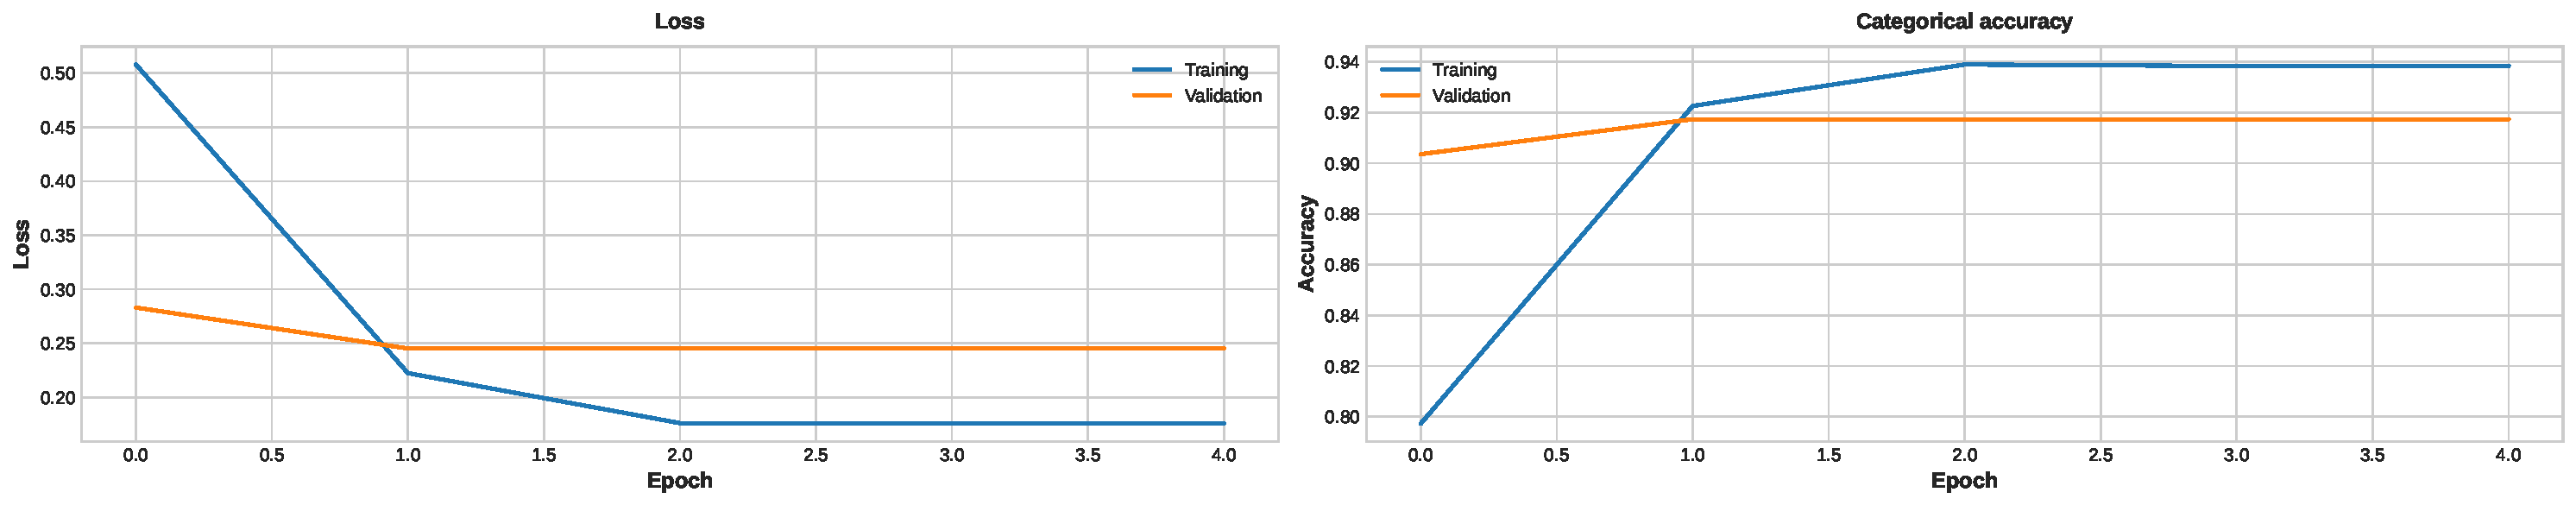
\includegraphics[width=18cm, height=9cm]{../results/desc_stats/accuracy_3classes_2.pdf}
\end{figure}

\begin{figure}[H]
    \centering
    \caption{Confusion Matrix: BERT Base}
    \label{fig:conf_BERT_base}
    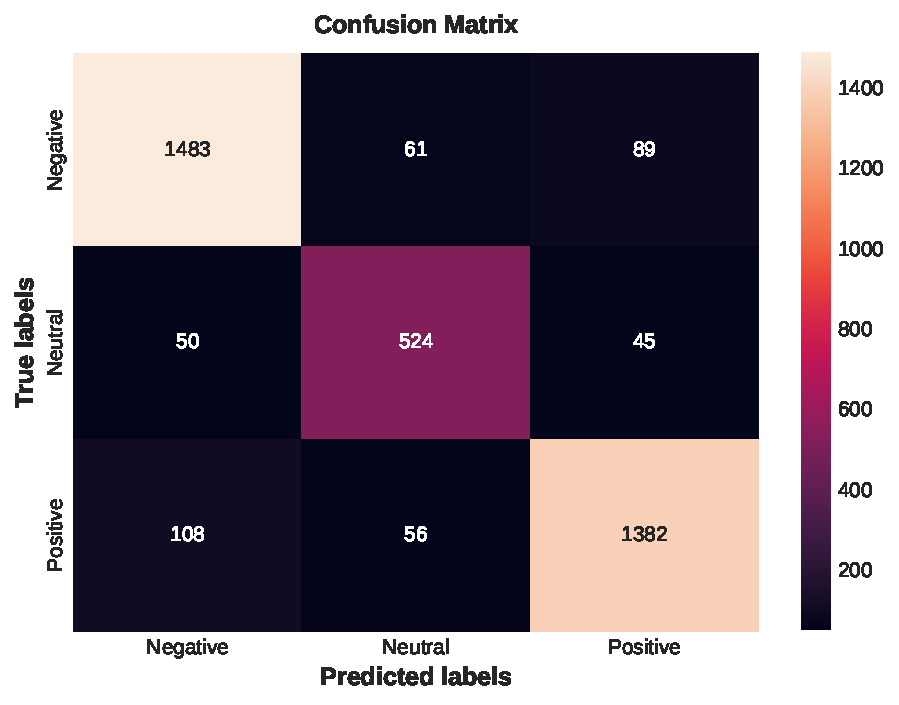
\includegraphics[width=14cm, height=10cm]{../results/desc_stats/confusion_3classes_2.pdf}
\end{figure}

\newpage


\subsection{First and Second Batch Content}
\label{app:pilot_content}
\begin{table}[ht]
		\centering
		\caption{\textbf{Africa Check Pilot Content: Kenya \label{tab:KE_1}}} 
		\begin{tabular}{|p{1cm}|p{7cm}|p{5cm}|}
			\hline
			Week & Suggested Text & Link to content \\ 
			\hline
			I & As technology advances so too has the speed and ease at which misinformation travels. To protect your friends and family, here are 5 questions to ask yourself before forwarding a message.      
            \#FactsMatter & Link: \href{https://www.dropbox.com/s/5gsfwz4tkv68q68/Africa_Check_message.mp4?dl=0}{5 Questions to Ask Before Forwarding a Message} \\ &  &\\
            I & A video shared online shows a brazen robbery and Kenyan social media users have claimed it illustrates the increase in crime in the capital Nairobi. But it’s from the South American country Guyana, not Kenya.                      
            \#FactsMatter & 
            Link: \url{https://africacheck.info/3OqcoqI}  \\ &  &\\
            II & The speed at which the Covid-19 vaccine was developed fueled understandable fears. But safety was not compromised - here’s why. \#FactsMatter & Link: \href{https://www.dropbox.com/s/qdm1q17izyxiwyl/Africa_Check_vaccine.mp4?dl=0}{The speed with which Covid-19 vaccine was developed did not compromise its safety.} \\ &  &\\
            II & Beware of Covid vaccine misinformation - a recent claim that Microsoft co-founder Bill Gates wants to “‘force-jab’ the unvaccinated” through vaccinated livestock is pure fabrication.  \#FactsMatter & Link: \url{https://africacheck.info/pfizer_employees} \\ &  &\\
            III & Seeing is believing? Not so fast. Here’s how to easily verify images and videos on social media and avoid being fooled by misinformation. \#FactsMatter & Link: \href{https://www.dropbox.com/s/kujk6fdjgasbkry/Africa_Check_youtube_image_220.mp4?dl=0}{Quick Steps to Verifying Videos or Images} \\ &  &\\
            III & A disturbing video of a girl being assaulted has been shared online with the claim the incident took place in Kenya. But the video was shot in the DRC. \#FactsMatter & Link: \url{https://africacheck.info/3RsXyBr} \\ &  &\\
            
   \hline
		\end{tabular}
  \end{table}
	\begin{table}[ht]
		\centering
  \caption{\textbf{Africa Check Content Plan: Kenya (Continued)} \label{tab:KE_2}}
		\begin{tabular}{|p{1cm}|p{7cm}|p{5cm}|}
			\hline
   IV & Heated arguments over dinner? Here’s what to do when your loved ones share misinformation, without upsetting them. \#FactsMatter & Link: \href{https://www.dropbox.com/s/s702vzeb8sc39ij/Africa_Check_misinformation.mp4?dl=0}{Dealing with family who share misinformation} \\ &  &\\
        IV & Have road crashes claimed more lives than Covid-19 in Kenya? Get the facts here:  
        \#FactsMatter
 & Link: \url{ https://africacheck.info/3jFojWA } \\ &  &\\
 V & Why do people create health disinformation? And what’s really the harm in sharing it? Keep your friends and family protected by looking out for these hidden motivations \#FactsMatter & Link: \href{https://www.dropbox.com/s/v8voe5fqa4b1fr2/Africa_Check_covid.mp4?dl=0}{Why do people share health misinformation?} \\ &  &\\
 V & While widespread antiretroviral treatment has drastically changed the lives of people with HIV, there is still no cure for the virus. Expensive treatments advertised on social media that claim otherwise should be ignored.
 \#FactsMatter
 & Link: \url{https://africacheck.info/fake_HIV_cure} \\ &  &\\
 VI & Here are @AfricaCheck’s top tips for spotting false information and stopping its spread
 \#FactsMatter & Link: \href{https://www.dropbox.com/s/wl2mzgkvqnw47dl/Africa_Check_youtube_fakenews.mp4?dl=0}{Top 4 tips to spot fake news} \\ &  &\\
 VI & A video claims that a Kenyan doctor has invented a cure for high blood pressure and is therefore in danger. The video includes the logo of KTN News and a clip of anchor Ali Manzu. But the channel – and Manzu – never reported this “news”.
 \#FactsMatter
 & Link: \url{https://africacheck.info/3WY6twP} \\ &  &\\
\hline
		\end{tabular}
\end{table}


	\begin{table}[ht]
		\centering
  \caption{\textbf{Africa Check Content Plan: Kenya  (Continued)} \label{tab:KE_3}}
		\begin{tabular}{|p{1cm}|p{7cm}|p{5cm}|}
			\hline
   VII & Medical advice and health tips are everywhere on social media. But some aren’t backed by science, and can even cause harm. These verification steps can help protect family and friends from health
misinformation
 \#FactsMatter & Link: \href{https://www.dropbox.com/s/b2bxkbjwtzp2xnr/Africa_Check_health.mp4?dl=0}{Verifying health claims quacks or false cures} \\ &  &\\
 VII & Some substances extracted from pineapples may help treat less serious conditions. But “hot pineapple water” definitely doesn’t cure cancer. This dangerous claim rehashes old (untrue) advice that “hot lemon water” cures cancer. \#FactsMatter
 & Link: \url{https://africacheck.info/3kGLAIe} \\ &  &\\
 VIII & IT’S A SCAM! Make sure you’re not fooled by using these simple steps.
 \#FactsMatter & Link: \href{https://www.dropbox.com/s/9gvyb2x4j09thiv/Africa_Check_facebook.mp4?dl=0}{Facebook scams and how to stop them} \\ &  &\\
 VIII & Beware of posts offering soft loans on WhatsApp from Kenya’s Family Bank. The loan terms are attractive. But the offer isn’t real, confirming that if something sounds too good to be true, it usually is. \#FactsMatter
 & Link: \url{https://africacheck.info/3lx7cHt} \\ &  &\\
\hline 
   \end{tabular}
\end{table}

\newpage

\begin{table}[ht]
		\centering
		\caption{\textbf{Africa Check First and Second Batch Content: South Africa \label{tab:SA_1}}} 
		\begin{tabular}{|p{1cm}|p{7cm}|p{5cm}|}
			\hline
			Week & Suggested Text & Link to content \\ 
			\hline
			I & As technology advances so too has the speed and ease at which misinformation travels. To protect your friends and family, here are 5 questions to ask yourself before forwarding a message.      
            \#FactsMatter & Link: \href{https://www.dropbox.com/s/5gsfwz4tkv68q68/Africa_Check_message.mp4?dl=0}{5 Questions to Ask Before Forwarding a Message} \\ &  &\\
            I & What do we know about race and private sector ownership in South Africa? Three viral claims are investigated here: 
            \#FactsMatter & 
            Link: \url{https://africacheck.info/3B86Trx} \\ &  &\\
            II & The speed at which the Covid-19 vaccine was developed fueled understandable fears. But safety was not compromised - here’s why. \#FactsMatter & Link: \href{https://www.dropbox.com/s/qdm1q17izyxiwyl/Africa_Check_vaccine.mp4?dl=0}{The speed with which Covid-19 vaccine was developed did not compromise its safety.} \\ &  &\\
            II & A claim that South Africans were given the “wrong Covid vaccine” is incorrect. A batch of nasal spray to help treat Covid symptoms was ordered by the defence department, but returned to Cuba after the public protector stepped in. \#FactsMatter & Link: \url{https://africacheck.info/3W19A6K} \\ &  &\\
            III & Seeing is believing? Not so fast. Here’s how to easily verify images and videos on social media and avoid being fooled by misinformation. \#FactsMatter & \href{https://www.dropbox.com/s/kujk6fdjgasbkry/Africa_Check_youtube_image_220.mp4?dl=0}{Quick Steps to Verifying Videos or Images} \\ &  &\\
            III & No, this photo doesn't show the British ambassador to Somalia with a black child in a cage.  \#FactsMatter & Link: \url{https://africacheck.info/british_ambassador_somalia} \\ &  &\\
            
   \hline
		\end{tabular}
  \end{table}

  
	\begin{table}[ht]
		\centering
     \caption{\textbf{Africa Check Content Plan: South Africa (Continued)} \label{tab:SA_2}}
		\begin{tabular}{|p{1cm}|p{7cm}|p{5cm}|}
			\hline
   IV & Heated arguments over dinner? Here’s what to do when your loved ones share misinformation, without upsetting them. \#FactsMatter & Link: \href{https://www.dropbox.com/s/s702vzeb8sc39ij/Africa_Check_misinformation.mp4?dl=0}{Dealing with family who share misinformation} \\ &  &\\
        IV & Is \#SouthAfrica’s much-criticised power utility @Eskom\_SA overstaffed by 66\%? And do salaries for 27,543 surplus staff amount to R1.38 billion per year? 
        These claims have been much shared online. But are they accurate? 
        \#FactsMatter
 & Link: \url{https://africacheck.info/eskom_salaries} \\ &  &\\
 V & Why do people create health disinformation? And what’s really the harm in sharing it? Keep your friends and family protected by looking out for these hidden motivations \#FactsMatter & Link: \href{https://www.dropbox.com/s/v8voe5fqa4b1fr2/Africa_Check_covid.mp4?dl=0}{Why do people share health misinformation?} \\ &  &\\
 V & While widespread antiretroviral treatment has drastically changed the lives of people with HIV, there is still no cure for the virus. Expensive treatments advertised on social media that claim otherwise should be ignored. \#FactsMatter
 & Link: \url{https://africacheck.info/fake_HIV_cure} \\ &  &\\
 VI & Here are @AfricaCheck’s top tips for spotting false information and stopping its spread
 \#FactsMatter & Link: \href{https://www.dropbox.com/s/wl2mzgkvqnw47dl/Africa_Check_youtube_fakenews.mp4?dl=0}{Top 4 tips to spot fake news} \\ &  &\\
 VI & Government ministers do sometimes put their feet in their mouths. But there’s no evidence South African minister of water \& sanitation suggested people shower ‘in groups’, however dire the country’s water and electricity crises might be.
 \#FactsMatter
 & Link: \url{https://africacheck.info/3U7Flt3} \\ &  &\\
\hline
		\end{tabular}
  \end{table}

  
	\begin{table}[ht]
		\centering
  \caption{\textbf{Africa Check Content Plan: South Africa (Continued)} \label{tab:SA_3}}
		\begin{tabular}{|p{1cm}|p{7cm}|p{5cm}|}
			\hline
   VII & Medical advice and health tips are everywhere on social media. But some aren’t backed by science, and can even cause harm. These verification steps can help protect family and friends from health
misinformation
 \#FactsMatter & Link: \href{https://www.dropbox.com/s/b2bxkbjwtzp2xnr/Africa_Check_health.mp4?dl=0}{Verifying health claims quacks or false cures} \\ &  &\\
 VII & Some substances extracted from pineapples may help treat less serious conditions. But “hot pineapple water” definitely doesn’t cure cancer. This dangerous claim rehashes old (untrue) advice that “hot lemon water” cures cancer.
  \#FactsMatter & Link: \url{https://africacheck.info/3kGLAIe} \\ &  &\\
 VIII & IT'S A SCAM! Make sure you're not fooled by using these simple steps.
 \#FactsMatter & Link: \href{https://www.dropbox.com/s/9gvyb2x4j09thiv/Africa_Check_facebook.mp4?dl=0}{Facebook scams and how to stop them} \\ &  &\\
 VIII & Beware of rings sold with the promise of weight loss or health benefits. It’s a scam, confirming that if something sounds too good to be true, it usually is.
  \#FactsMatter
 & Link: \url{https://africacheck.info/3wphJGV} \\ &  &\\
\hline 
   \end{tabular}
\end{table}
